\documentclass{beamer}
\usepackage{pgfpages}

\setbeameroption{show notes}
\setbeameroption{show notes on second screen=right}
\setbeamerfont{note page}{size=\tiny}

\usepackage[latin1]{inputenc}
\usepackage[T1]{fontenc}
\usepackage[english]{babel}
\usepackage{lmodern}
%\usepackage[pdftex]{graphicx}
\usepackage{standalone}
\usepackage{tikz,pgfplots}
\usepgfplotslibrary{groupplots}
\usepgfplotslibrary{units} 
\usetikzlibrary{patterns}
\usetikzlibrary{arrows}
\usetikzlibrary{shapes.arrows}
\usetikzlibrary{shapes.symbols}

\pgfplotsset{
            compat={1.3},
            legend style={
                        cells={anchor=west},
                        legend pos=outer north east},
            cycle list name=linestyles,
            axis x line=center, %bottom,
            axis y line=center, %left,
            enlarge x limits=0.1,
            enlarge y limits=0.2,
            samples = {50},
            samples y= {50}
            %enlarge x limits={value=0.1, upper},
            %axis equal=true,
            %axis equal image = true,

} 

\title{Robust Optimization}
\author{Annkathrin Kr\"{a}mmer, Sabina Przioda, Christian Kreipl, Johannes Milz}
\date{May 27, 2015}
\institute{Technische Universit\"{a}t M\"{u}nchen}




%-----------------------------------------

\setbeamertemplate{footline}[frame number]
\usecolortheme{rose}
\useinnertheme[shadow]{rounded}


%\include{structure.tex}

\usepackage{marvosym}

\begin{document}

\maketitle

%------------------------------------------


\begin{frame}
\frametitle{Contents}
\tableofcontents
\note{

\begin{itemize}
\item Our work is divided into 4 parts
\begin{itemize}
\item Model of a Car
\item Mathematical problem formulation
\item Implementation 
\item Visualization
\end{itemize}
\end{itemize}


}
\end{frame}

%------------------------------------------


\section{Motivation}


\begin{frame}
\frametitle{Motivation}


\begin{itemize}
\item steering a car 
\item minimize fuel consumption
\item constraints
\begin{itemize}
\item avoid crashes
\item dynamics
\end{itemize}
\end{itemize}
\begin{block}{Problem}
Dynamics change considerably, e.g., for different weather.
\bigskip \\
\MVRightarrow \ Robust Optimization
\end{block}

\note{
\begin{itemize}
\item Our goal is to steer a car such that the fuel consumption is minimal 
\item Contraints: Avoid Crashes
\begin{itemize}
\item our car is not allowed to leave the road
\item hit other cars or construction sites
\end{itemize}
\item Dynamics of the car
\begin{itemize}
\item motion of the car
\begin{itemize}
\item slipping behavior 
\item acceleration behavior
\end{itemize}
\end{itemize}
\item Problem: Changing weather has a major impact on the slipping behavior
\begin{itemize}
\item we cannot drive fast on icy roads
\item Rain causes aquaplaning
\end{itemize}
\item Way out: Robust Optimization
\begin{itemize}
\item This Optimization method takes changing parameters such as weather into account.
\item Car is steered save for changing conditions such as weather, different roads...
\end{itemize}
\end{itemize}
}



\end{frame}





%------------------------------------------

\section{Model of Car}


\begin{frame}
\frametitle{Model of Car}


\begin{figure}[T]
\centering
\includestandalone[angle = -10, width=0.8\textwidth]{cartikz}
\end{figure}





\note{
\begin{itemize}
\item Our car is described as a pointmass, for simplicity
\item Road is visualized in gray
\item Car as a rectangle
\item steering angle is denoted by $\beta(t)$
\begin{itemize}
\item We applied Newton's mechanic
\item The motion/ direction of motion is described with 
\begin{itemize}
\item The steering angle $\beta(t)$
\item The acceleration force pushing the car forward 
\item The central forces 
\item If the speed of the car is to high, it slides and may leave the road.
\end{itemize}
\end{itemize}
\end{itemize}
}

\end{frame}

\begin{frame}
\frametitle{Dynamical System}

\begin{block}{}
\begin{align*}
& \dot{x}(t) = G(x(t), u(t), p) & x(0) = x_0,
\end{align*}
where 
\begin{align*}
& x \in C^1([0, t_f], \mathbb{R}^{n}) \text{ is the state variable,}\\
& u \in C^1([0, t_f], \mathbb{R}^{m}) \text{ is the control variable,}\\
& p \in \mathbb{R}^{n_p} \text{ is the uncertain parameter vector.}
\end{align*}
\end{block}

\note{
\begin{itemize}
\item Motion of the car is described as a dynamical system, i.e., with a ODE and an initial value
\item $t_f$ is the final time
\item our states: path, velocity, steering angle
\item control: brake, motor torque (gas petal), steering angle velocity
\item parameter: weather, rolling friction coefficients, uncertain sea level due to wrong NAVI data
\end{itemize}
}
\end{frame}

%------------------------------------------

\section{Optimal Control Problem}




\begin{frame}
\frametitle{Optimal Control Problem}
\begin{block}{}
\begin{align*}
 &&& \min_{x(\cdot)\in \mathbb{R}^{n_{x}}, u(\cdot)\in \mathbb{R}^{n_{u}}}  f_{0}(x, u)\\
& \text{ s.t. } && \dot{x}(t) = G(x(t), u(t), p) && \forall t \in [0, t_f],\\
&&& x(0) = x_0,\\
&&&  f_{i}(x(t),u(t)) \leq 0 & \text{ for } & i=1,\ldots,n_{f},\\
 &&&&& \forall t \in [0, t_f].
\end{align*}
\end{block}
\end{frame}


%------------------------------------------


\section{Discretization}


\begin{frame}
\frametitle{Discretization}
\begin{itemize}[<+->]
\item infinte dimensional optimization problem
\item $\Rightarrow$ approximate the optimal control problem by a discretization
\begin{figure}
\centering
\includestandalone[width=0.8\textwidth]{TikzDiscretization}
\end{figure}
\end{itemize}




\end{frame}


\begin{frame}
\frametitle{Multiple Shooting}
\only<1>{
\begin{figure}
\centering
\includestandalone[width=0.8\textwidth]{TikzMultiShooti1}
\end{figure}
% Bild von Johannes einfügen was Multiple shooting zeigt OHNE Steuerung
}
\only<2>{
\begin{figure}
\centering
\includestandalone[width=0.8\textwidth]{TikzMultiShooti2}
\end{figure}

% Bild von Johannes einfügen was Multiple shooting zeigt MIT Steuerung
}
\only<3>{\begin{figure}
\centering
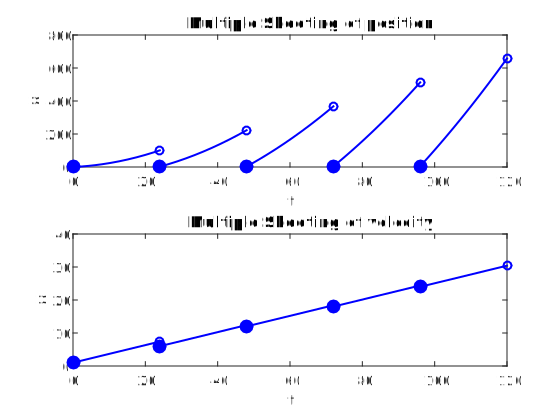
\includegraphics[width=0.9\textwidth]{Sabina/MultipleShooting21.pdf}
\end{figure}}
\only<4>{\begin{figure}
\centering
\includegraphics[width=0.9\textwidth]{Sabina/MultipleShooting24.pdf}
\end{figure}}
\only<5>{\begin{figure}
\centering
\includegraphics[width=0.9\textwidth]{Sabina/MultipleShooting27.pdf}
\end{figure}}
\only<6>{\begin{figure}
\centering
\includegraphics[width=0.9\textwidth]{Sabina/output4.pdf}
\end{figure}}
\end{frame}

%------------------------------------------

\section{Robust Optimization Problem}



\begin{frame}
\frametitle{Constraints for Parameters}

\begin{block}
	
\begin{align*}
 &&& \min_{x\in \mathbb{R}^{n_{x}}, u\in \mathbb{R}^{n_{u}}}  f_{0}(x, u)\\
& \text{ s.t. } &&  f_{i}(x,u) \leq 0 & \text{ for } & i=1,\ldots,n_{f}\\
&&&  g_{j}(x,u,p)=0 & \text{ for } & j=1,\ldots,n_{x},
\end{align*}
where $p\in \mathbb{R}^{n_{p}}$ is an uncertain parameter vector.

\end{block}


\begin{block}

\begin{equation*}
\mathbb{P}_{box}=\left\{\left. p \right| p_{l}\leq p \leq p_{u}\right\}
\end{equation*}
$p_{l}$: lower bound, $p_{u}$: upper bound
\begin{align*}
& \text{weather: }  & \left\{\left. p \right| 0\leq p\leq 1\right\} \\
& \text{height profil: } & \left\{\left. p \right| 0\leq p\leq 45\right\}
\end{align*}


\end{block}

\note{
I think this might not be clear: Both, the weather and height are $\in \mathbb{R}^{n_p}$ or not necessarily the same dimension? Later, you write $p in \mathbb{P}_{box}$
}

\end{frame}


%<<<<<<< HEAD
\begin{frame}
\frametitle{Worst Case Formulation}

EXAMPLE?

\begin{align*}
&&&\Phi_{i}(u)=\max_{x\in \mathbb{R}^{n_{x}}, p\in \mathbb{R}^{n_{p}}} f_{i}(x,u)\\
	& \text{s.t. } && g(x,u,p)=0\\
	&&& p\in\mathbb{P}_{box}
\end{align*}

\begin{block}{Robust Counterpart}
\begin{align*}
&&&\min_{u\in\mathbb{R}^{n_{u}}} \Phi_{0}(u)\\
&\text{s.t. } &&\Phi_{i}(u)\leq 0 & \text{ for } & i=1,\ldots,n_{f}.
\end{align*}
$\Rightarrow$ bilevel structure!
\note{
I would not write the remark down.
}
\end{block}

\end{frame}

\begin{frame}
	\frametitle{Approximation Technique}

\begin{block}{Linearization}
	\begin{align*}
	&&&\tilde{\Phi}_{i}(u)=\max_{(x-\bar{x})\in\mathbb{R}^{n_{x}}, (p-\bar{p})\in\mathbb{R}^{n_{p}}} f_{i}(\bar{x}, u)+\frac{\partial f_{i}}{\partial x}(\bar{x}, u)(x-\bar{x})\\
	&\text{s.t.} && \frac{\partial g}{\partial x}(\bar{x}, u, \bar{p})(x-\bar{x})+\frac{\partial g}{\partial p}(\bar{x}, u, \bar{p})(p-\bar{p})=0\\
	&&&p-\bar{p} s.th. p\in\mathbb{P}_{box}
	\end{align*}
	
	\note{
	Might not be clear what s.th. means	
	}
\end{block}	
	

	
\begin{block}	

\begin{align*}
&&&\min_{u\in\mathbb{R}^{n_{u}}, \bar{x}\in\mathbb{R}^{n_{x}}} \tilde{\Phi}_{0}(u)\\
&\text{s.t.} &&  \tilde{\Phi}_{i}(u)\leq 0 & \text{ for } & i=1,\ldots,n_{f}\\
&&&g(\bar{x}, u, \bar{p})=0
\end{align*}
\end{block} 
	
$\Rightarrow$ Standard Optimization Problem (SQP or else)

\note{
I would not write this commend down. (5 times 5 rule ;)
}
\end{frame}
%=======
%>>>>>>> origin/master


%------------------------------------------



\section{Visualization}

\begin{frame}
\frametitle{Visualization}

	\only<1>{
	What do we want?
	}
	\only<2>{
	\begin{itemize}
		\item sell our results to you

		\item nice graphs

		\item rendered video
	\end{itemize}
	}
	
	\only<3>{
	What can we improve?
	}

	\only<4>{
	\begin{itemize}

		\item textures

		\item nonlinear street design

		\item fit acceleration to optimization results

		\item fit resolution to output device

		\item follow the car with the camera
	\end{itemize}
	}
	\note{
		\begin{itemize}
			\item graphs contain much information
			\item videos catch people where they are
		\end{itemize}
	}

	\note{
		\begin{itemize}

			\item Graphs are graphs, nothing to do here
			\item Grass tiles
			\item Make car shiny, windows glassy
			\item Curves are nice to see
			\item this is just an arbitrary acceleration
			\item This 10 seconds clip allready rendered 30 min
			\item min 18FPS needed

		\end{itemize}


}

\end{frame}







%------------------------------------------


\bibliography{lit.bib}

\end{document}



